\documentclass{beamer}
\usepackage[T1]{fontenc}
\usepackage{textcomp}
\usepackage[utf8x]{inputenc}
\usepackage[british]{babel}
\usepackage{url}
\usepackage{listings}
\usepackage{graphicx}
%\usepackage{soul}

%FONT
\usepackage{bera}
\usepackage[garamond]{mathdesign}
\renewcommand{\rmdefault}{ugm} % garamond
\renewcommand{\sfdefault}{ugm} % sans-serif font

% must be included after hyperref (and float)
% \usepackage[noend]{algorithmic}
% \usepackage{algorithm}
% \usepackage[noend]{algpseudocode}

\title{Fitting an All-atom Protein Model to a $C_{\alpha}$-trace}

\author{\small Martin Dybdal \and Anders Boesen Lindbo Larsen \and Esben Skaarup}

\institute{\textrm{Datalogisk Institut, Københavns Universitet}}
\date{\today}

\mode<presentation>
{
  \usetheme{Frankfurt}
  %\usetheme{Warsaw} 
  \definecolor{uofsgreen}{rgb}{.125,.5,.25}
  \definecolor{natvidgreen}{rgb}{.196,.364,.239}
  \definecolor{kugrey}{rgb}{.4,.4,.4}
  \usecolortheme[named=uofsgreen]{structure}
  \usefonttheme[onlylarge]{structuresmallcapsserif}
  \usefonttheme[onlysmall]{structurebold}
}

\logo{
\includegraphics[height=1.5cm]{diku.png}}

\usenavigationsymbolstemplate{} % fjern navigation

\setcounter{tocdepth}{1}

\begin{document}

\frame{\titlepage}

% Martin
\section{Introduction}
\subsection{Protein structure}
\begin{frame}[t, fragile]
  \frametitle{Protein structure prediction}

  \begin{block}{blok}
    a
  \end{block}

  \pause

  \begin{itemize}
    \item 1
    \item 2
  \end{itemize}

\end{frame}

% Anders


% Esben

\section{Fitting Side-chains}

\subsection{dummy}
\begin{frame}
	\frametitle{Rotamers}
	
	\begin{itemize}
		\item Rotamer
		\begin{itemize}
			\item Amino acid with set of $\chi$ angles
			\item Probabilities
		\end{itemize}
		\item Dunbrack
		\begin{itemize}
			\item Open license
			\item Widely used
			\item Simple format
		\end{itemize}
	\end{itemize}
	
\end{frame}

\subsection{dummy}
\begin{frame}
	\frametitle{Collision detection}
	
	\begin{itemize}
		\item Implicit H-atoms
		\item No description in literature
		\item Fixed collision distance: 1.25 Å
		\begin{itemize}
			\item Larger distance would causes collisions in known protein structures
			\item Smaller distance would cause the structure to become sparse
		\end{itemize}
	\end{itemize}
	
\end{frame}

\subsection{dummy}
\begin{frame}
	\frametitle{Algorithm}
	\begin{columns}[c]
	\column{5.5cm}
	
	% \begin{algorithm}
	% % \caption{Overview of the general algorithm using leapfrogging}
	% \begin{algorithmic}
	% 	\FOR{each side-chain}
	% % 	% 	\STATE Reset $\chi$ angles
	% % 	% \ENDFOR
	% % 	% \FOR{each side-chain}
	% % 	% 	\FOR{each colliding side-chain}
	% % 	% 		\STATE Resolve recursively
	% % 	% 	\ENDFOR
	% 	\ENDFOR
	% \end{algorithmic}
	% \end{algorithm}
	
	% \begin{lstlisting}
	\texttt{For each side-chain}\\
	\texttt{\;\;\;\;Reset $\chi$ angles}\\
	\texttt{For each side-chain}\\
	\texttt{\;\;\;\;For each colliding side-chain}\\
	\texttt{\;\;\;\;\;\;\;\;Resolve recursively}\\
 	% \end{lstlisting}

	% For each side-chain
	% 	Reset $\chi$ angles
	% For each side-chain
	% 	For each colliding side-chain
	% 		Resolve recursively

	% \begin{itemize}
	% 	\item For each side-chain
	% 	\begin{itemize}
	% 		\item Reset $\chi$ angles
	% 	\end{itemize}
	% 	\item For each side-chain
	% 	\begin{itemize}
	% 		\item For each colliding side-chain
	% 		\begin{itemize}
	% 			\item Resolve recursively
	% 		\end{itemize}
	% 	\end{itemize}
	% \end{itemize}
	
% \end{frame}

% \begin{frame}
	% \frametitle{Algorithm}
	
	\column{5cm}
	\begin{figure}
		% \centering
		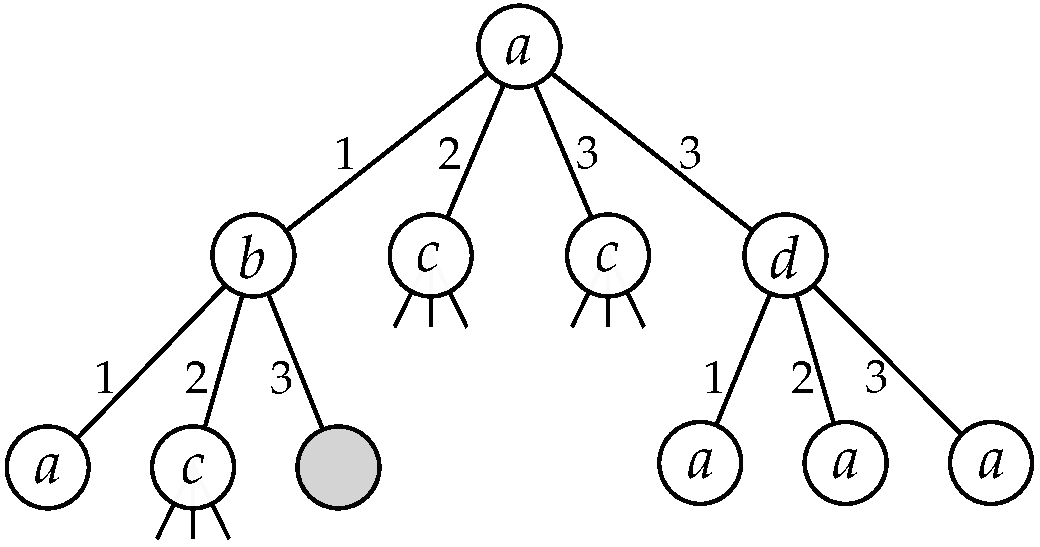
\includegraphics[width=5cm]{../rapport/figures/rotamersearch.pdf}
	\end{figure}
	
	\end{columns}
\end{frame}

\subsection{dummy}
\begin{frame}
	\frametitle{Performance}
	
	\begin{itemize}
		\item Backbone fitting quality affects side-chain collisions
		\item Fitting resolves $4/5$ collisions
		\item Some collision can not be solved
		\begin{itemize}
			\item Proline collides with backbone
			\item Side-chains are placed too close to each other
		\end{itemize}
		\item Collision depth of 3 seems optimal
	\end{itemize}
	
\end{frame}

\subsection{dummy}
\begin{frame}
	\frametitle{Performance}
	
	\begin{figure}
		\centering
		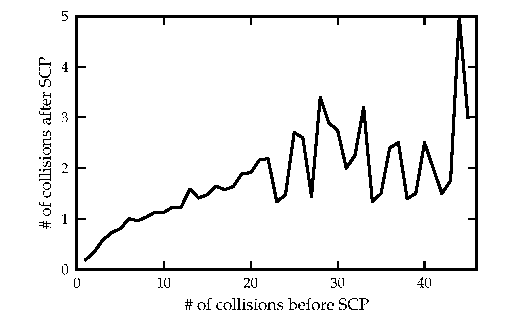
\includegraphics[width=.75\columnwidth]{../rapport/figures/plot_scp}
	\end{figure}
	
\end{frame}


\section{Conclusion}

\subsection{dummy}
\begin{frame}
	\frametitle{Conclusion}
	Det endte godt alligevel
\end{frame}


\end{document}
